\documentclass[12pt]{article}
\usepackage{amssymb, amsmath, amsthm, amsfonts}
\usepackage[alphabetic]{amsrefs}
\usepackage{mathrsfs,comment}
\usepackage{float}
\usepackage{bm}
\usepackage{subcaption}
\usepackage[all,arc,2cell]{xy}
\usepackage{enumerate}
\usepackage{url}
\usepackage{tcolorbox}
\usepackage[margin=0.75in]{geometry}
\usepackage{listings}
\usepackage{MnSymbol}
\usepackage{pdfpages}
\usepackage{tikz}
\usetikzlibrary{arrows,automata,calc,positioning}
\usepackage[colorlinks = true,
linkcolor = blue,
urlcolor  = blue,
citecolor = blue,
anchorcolor = blue]{hyperref}

\usepackage{cleveref}


%theoremstyle{plain} --- default
\newtheorem{theorem}{Theorem}[section]
\newtheorem{corollary}[theorem]{Corollary}
\newtheorem{conjecture}[theorem]{Conjecture}
\newtheorem{proposition}[theorem]{Proposition}
\newtheorem{lemma}[theorem]{Lemma}

\theoremstyle{definition}
\newtheorem{definition}[theorem]{Definition}
\newtheorem{example}[theorem]{Example}
\newtheorem{remark}[theorem]{Remark}
\newtheorem*{solution}{Solution}


\makeatother
\numberwithin{equation}{section}



%%%Commands and shortcuts%%%%
%

\newcommand{\R}{\mathbb{R}}
\newcommand{\Q}{\mathbb{Q}}
\newcommand{\Z}{\mathbb{Z}}
\newcommand{\N}{\mathbb{N}}
\newcommand{\F}{\mathbb{F}}
\newcommand{\xb}{\mathbf{x}}
\newcommand{\yb}{\mathbf{y}}
\newcommand{\ab}{\mathbf{a}}
\newcommand{\zb}{\mathbf{z}}
\newcommand{\func}[3]{#1\colon #2 \rightarrow #3}
\newcommand{\sumn}{\sum_{i=1}^{n}}
\newcommand{\innerp}[2]{\langle #1,#2 \rangle}
\newcommand{\dsq}{d_{sq}}
\newcommand{\dtc}{d_{tc}}
\newcommand{\ifff}{if and only if }
\newcommand{\st}{such that }
\newcommand{\te}{there exists }
\newcommand{\wrt}{with respect to }
\newcommand{\wloG}{without loss of generality }
\newcommand{\Wlog}{Without loss of generality }
\newcommand{\ssteq}{\subseteq}
\newcommand{\setst}{\hspace{1mm} | \hspace{1mm} }
\newcommand{\Bs}{\mathscr{B}}
\newcommand{\Us}{\mathscr{U}}
\newcommand{\T}{\mathcal{T}}
\newcommand{\Y}{\mathcal{Y}}
\newcommand{\B}{\mathcal{B}}
\newcommand{\G}{\mathcal{G}}
\newcommand{\Pc}{\mathcal{P}}
\newcommand{\Sc}{\mathcal{S}}
\newcommand{\C}{\mathcal{C}}
\newcommand{\A}{\mathcal{A}}
\newcommand{\Lc}{\mathcal{L}}
\newcommand{\onen}{\{1,\ldots,n\}}
\newcommand{\finv}[2]{#1^{-1}\left(#2\right)}		
\newcommand{\es}{\varnothing}	
\newcommand{\ol}[1]{\overline{#1}}	
\newcommand{\xnn}{(\mathbf{x}_n)_{n \in \N}}
\newcommand{\sft}{\mathbf{SFT_1}}		
\newcommand{\cop}{\sqcup}	
\newcommand{\cyc}[1]{#1_1\ldots #1_n#1_1}	
\newcommand{\pcyc}[2]{#2(#1_1)\ldots #2(#1_n)#2(#1_1)}	
\newcommand{\cyci}[2]{#1_1\ldots #1_{#2}#1_1}
\newcommand{\pcyci}[3]{#3(#1_1)\ldots #3(#1_{#2})#3(#1_1)}
\newcommand{\xh}{\bar{x}}	
\newcommand{\yh}{\bar{y}}		
\newcommand{\equivcls}[1]{#1/{\sim}}	
\newcommand{\modab}[3]{#1 \equiv #2 \pmod{#3}}						
\newcommand{\farg}{{-}}		
\newcommand{\uvec}[1]{\boldsymbol{\hat{\textbf{#1}}}}																																				

\DeclareMathOperator{\Cl}{Cl}
\DeclareMathOperator{\Bd}{Bd}
\DeclareMathOperator{\Int}{Int}
\DeclareMathOperator{\id}{id}
\DeclareMathOperator{\Hom}{Hom}
\DeclareMathOperator{\Tor}{Tor}
\DeclareMathOperator{\Ext}{Ext}

\renewcommand{\epsilon}{\varepsilon}
%\renewcommand{\phi}{\varphi}
\renewcommand\qedsymbol{$\blacksquare$}

\usepackage{color}
\newcommand{\Comments}{1}
\newcommand{\raf}[1]{\ifnum\Comments=1\textcolor{blue}{[RF: #1]}\fi}


\title{CSCI 5636 Final Project\\
\large A finite-element approach simulating flow over an airfoil using FEniCS}
\author{Luke Meszar}
\date{\today}
\begin{document}
	\maketitle
	\section*{Introduction}
	In this project, I set up a simulation for flow over an airfoil. I used the open source finite-element software FEniCS \cite{AlnaesBlechta2015a} to set up the simulations. The goal was to simulate low Reynolds number flow over an airfoil and calculate the lift and drag with various angles of attack. 
	\section*{Methodology}
	\setcounter{section}{1}
	The NACA 5012 airfoil was used for this simulation. The NACA airfoil series  \cite{marzocca2009naca} is a simple way to describe the geometry of an airfoil. In the four-digit series, the first two numbers describe the maximum camber as a percentage of the maximum chord length and the last two numbers describe the maximum thickness as a percentage of the chord length. This airfoil can be described by a series of Cartesian coordinates. Using the \textit{dat2gmsh.py} script found \href{http://community.dur.ac.uk/g.l.ingram/download.php}{here.} I was able to convert to a format that was readable by GMSH. GMSH \cite{geuzaine2009gmsh} is an open source geometry and meshing tool. Once I created a mesh \cref{fig:mesh} in GMSH I was able to export it to a format readable by FEniCS using their tool \textit{dolfin-convert.}
	\begin{figure}[H]
		\centering
		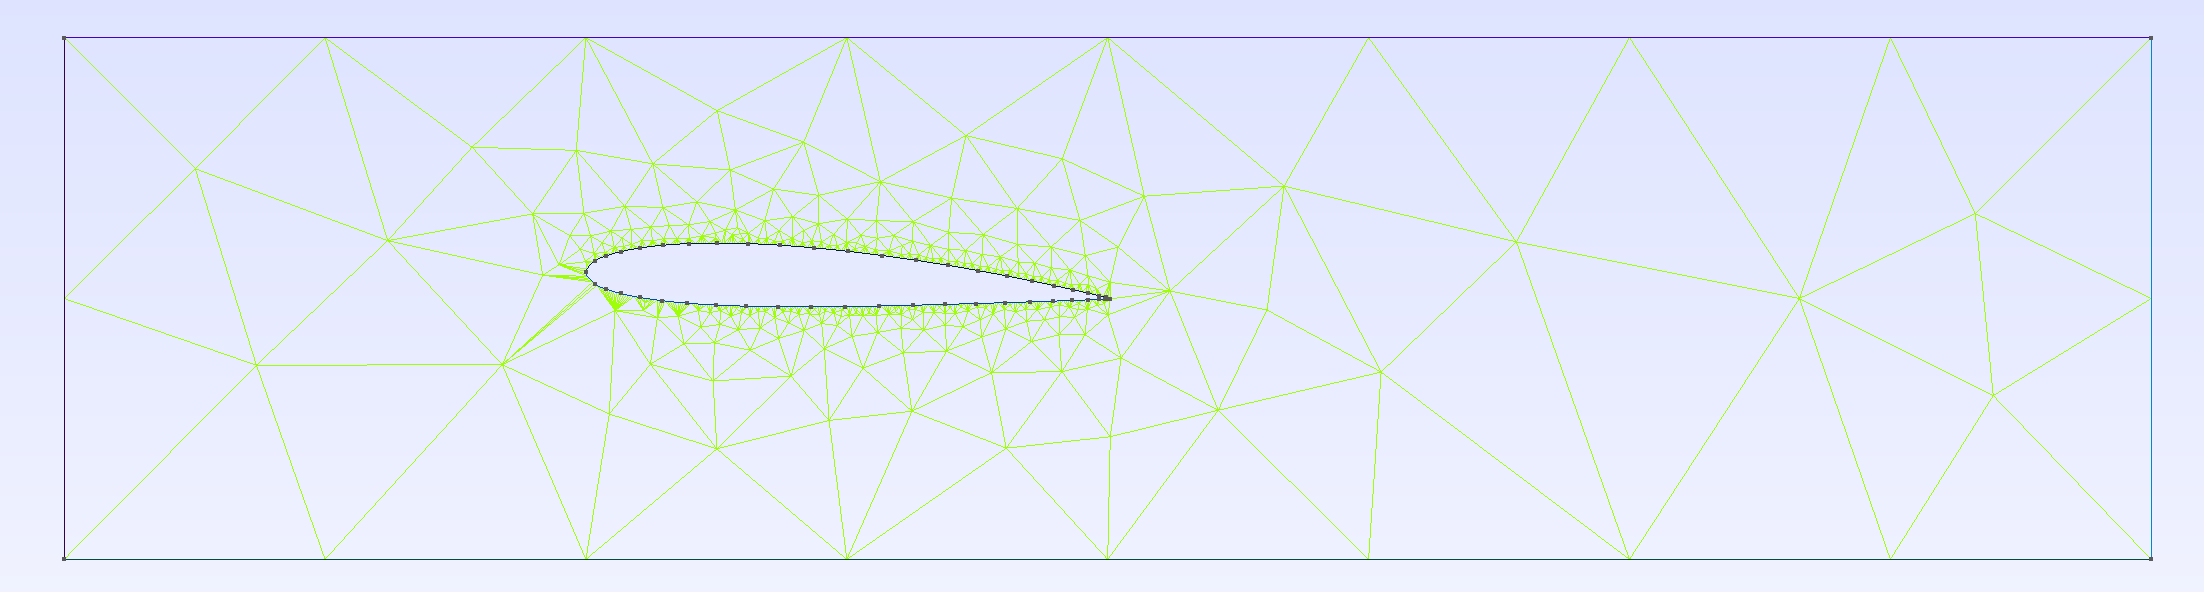
\includegraphics[scale=0.2]{airfoil_mesh.png}
		\caption{Mesh of the NACA 5012 Airfoil}
		\label{fig:mesh}
	\end{figure}

	Now that I had an xml file of the mesh, I was able to write a script that generated the subdomains of the mesh. By assigning different numbers to each region, I was able to partition the mesh. I created a different domain for the interior, the boundary of the airfoil, the left wall, the right wall, and the top and bottom walls. The code I used for this is in \textit{generate\_subdomains.py} which can be found in the appendix. 
	
	Now that the mesh has been generated and the necessary subdomains marked, a numerical solution can be computed. For this problem, I solved the following incompressible form of the Navier-Stokes equation:
	\begin{align}
	&\rho\left(\frac{\partial u}{\partial t} + u \cdot \nabla u\right) = \nabla\cdot \sigma(u,p) + f \\
	&\nabla \cdot u = 0
	\end{align}
	for the velocity $u$ and the pressure $p$. Here $\rho$ is the density of liquid and $f$ is the external body forces. Finally, $\sigma(u,p)$ is the stress tensor given by 
	\begin{equation}
	\sigma(u,p)=2\mu\epsilon(u)-pI
	\end{equation}
	where $\mu$ is the dynamic viscosity and $\epsilon(u)$ is the strain-rate tensor
	\begin{equation}
	\epsilon(u) = \frac{1}{2}\left(\nabla u + (\nabla u)^T\right).
	\end{equation}
	
	To solve this system of equations using a finite-element method, it will have to be converted to a weak form first. Due to the inherent structure of these equations, a simple finite-difference method at each timestep will not work. Instead the method known as IPCS \cite{goda1979multistep} (Incremental Pressure Correction System) will be used. 
	
	At each timestep, we will have to eventually update the values for the velocity and pressures. The IPCS method starts by estimating a tentative velocity $u^*$ using a midpoint finite-difference scheme as
	\begin{equation}\label{eq:tenvel}
	\langle\rho(u^*-u^n)/\Delta t,v\rangle+\langle\rho u^n\cdot\nabla u^n,v\rangle+\langle \sigma(u^{n+\frac{1}{2}},p^n),\epsilon(v)\rangle+\langle 	p^nn,v\rangle_{\partial\Omega}-\langle \mu\nabla u^{n+\frac{1}{2}}\cdot n,v\rangle_{\partial\Omega}=\langle f^{n+1},v\rangle
	\end{equation}
	with the notation
	\begin{align*}
	&\langle v,w\rangle=\int_\Omega vw\,dx\\
	&\langle v,w\rangle_{\partial\Omega} = \int_{\partial\Omega}vw\,ds.
	\end{align*}
	Now, we move on to compute the new pressure using the tentative velocity $u^*$ as
	\begin{equation}\label{eq:newpress}
	\langle\nabla p^{n+1},\nabla q\rangle=\langle\nabla p^n,\nabla q\rangle-\Delta t^{-1}\langle\nabla\cdot u^*,q\rangle.
	\end{equation}
	Finally, to compute the new velocity we use
	\begin{equation}\label{eq:newvel}
	\langle u^{n+1},v\rangle=\langle u^*,v\rangle-\Delta t\langle\nabla(p^{n+1}−p^n),v\rangle.
	\end{equation}
	Now, to show how to implement this method into FEniCS. 
	\begin{lstlisting}[language=Python]
	V = VectorFunctionSpace(mesh, 'CG', 2)
	Q = FunctionSpace(mesh, 'CG', 1)
	\end{lstlisting}
	We create a finite-element space for the velocity and pressure of dimension two and one respectively. This defines a domain consisting of Taylor-Hood elements needed for stability for these equations. 
	
	Next, we create the boundary conditions. We choose to have the left, top, and bottom walls have flow defined by the vector $U_0\cos(\theta)\uvec{i} + U_0\sin(\theta)\uvec{j}$. By varying $\theta$, different angles of attack of the wing can be simulated. The boundary of the airfoil is given a noslip boundary condition. The outflow is given a constant value of 0 for the pressure.
	
	\begin{lstlisting}[language=Python]
	theta = float(sys.argv[1])
	U_0 = 1.0
	u_outer_boun = Constant((U_0*cos(theta), U_0*sin(theta)))
	noslip = Constant((0, 0))
	
	#airfoil
	bcu_airfoil = DirichletBC(V, noslip, sub_domains, 0) 
	#top and bottom walls
	bcu_top_bot = DirichletBC(V, u_outer_boun, sub_domains, 3)
	#left wall
	bcu_inflow = DirichletBC(V, u_outer_boun, sub_domains, 1)
	#right wall 
	bcp_outflow = DirichletBC(Q, Constant(0), sub_domains, 2) 
	\end{lstlisting}
	
	Then the necessary trial and test functions and other parameters necessary to set up the weak form equations are defined. In the code $u_{\_}$ takes the place of $u^{n+1}$ and $u_{\_n}$ takes the place of $u^n$ from above. 
	
	\begin{lstlisting}[language=Python]
	u = TrialFunction(V)
	v = TestFunction(V)
	p = TrialFunction(Q)
	q = TestFunction(Q)
	
	u_n = Function(V)
	u_  = Function(V)
	p_n = Function(Q)
	p_  = Function(Q)
	
	
	
	U  = 0.5*(u_n + u)
	n  = FacetNormal(mesh)
	f  = Constant((0, 0))
	k  = Constant(dt)
	mu = Constant(mu)
	rho = Constant(rho)
	
	def epsilon(u):
	return 0.5*(nabla_grad(u) + nabla_grad(u).T)
	
	def sigma(u, p):
	return 2*mu*epsilon(u) - p*Identity(len(u))
	
	dx = Measure("dx", domain=mesh, subdomain_data=sub_domains)
	ds = Measure("ds", domain=mesh, subdomain_data=sub_domains)
	\end{lstlisting}
	
	Now, we can definition the variation equations for the weak form:
	\begin{lstlisting}[language=Python]
	F1 = rho*dot((u - u_n) / k, v)*dx \
	+ rho*dot(dot(u_n, nabla_grad(u_n)), v)*dx \
	+ inner(sigma(U, p_n), epsilon(v))*dx \
	+ dot(p_n*n, v)*ds - dot(mu*nabla_grad(U)*n, v)*ds \
	- dot(f, v)*dx
	a1 = lhs(F1)
	L1 = rhs(F1)
	
	a2 = dot(nabla_grad(p), nabla_grad(q))*dx
	L2 = dot(nabla_grad(p_n), nabla_grad(q))*dx -
	(1/k)*div(u_)*q*dx
	
	a3 = dot(u, v)*dx
	L3 = dot(u_, v)*dx - k*dot(nabla_grad(p_ - p_n), v)*dx
	\end{lstlisting}
	
	Here $a1$ and $L1$ correspond to \cref{eq:tenvel}, $a2$ and $L2$ correspond to \cref{eq:newpress} and $a3$ and $L3$ correspond to \cref{eq:newvel}.
	
	Next, we define the functional forms for drag and lift as
	\begin{lstlisting}[language=Python]
	D = p*n[0]*ds(0)
	L = p*n[1]*ds(0)
	\end{lstlisting}
	
	For lift we want to find the contribution of the pressure in the upwards direction and for drag we want to find it in the left to right direction. 
	
	Finally, we come to the timestep loop.
	\begin{lstlisting}[language=Python]
	t = 0
	for n in range(num_steps):
		# Update current time
		t += dt
		
		# Step 1: Tentative velocity step
		b1 = assemble(L1)
		[bc.apply(b1) for bc in bcu]
		solve(A1, u_.vector(), b1, 'bicgstab', 'ilu')
		
		# Step 2: Pressure correction step
		b2 = assemble(L2)
		[bc.apply(b2) for bc in bcp]
		solve(A2, p_.vector(), b2, 'cg', 'hypre_amg')
		
		# Step 3: Velocity correction step
		b3 = assemble(L3)
		solve(A3, u_.vector(), b3, 'bicgstab', 'ilu')
		
		drag_list.append(drag.inner(p_n.vector()))
		lift_list.append(lift.inner(p_n.vector()))
		time_list.append(t)
		
		# Update previous solution
		u_n.assign(u_)
		p_n.assign(p_)
	\end{lstlisting}
	
	For each solve, a Krylov method was used with a different iteration methods and preconditioners. At each time step, the lift and drag where computed by evaluating the necessary surface integrals.

	The full code can be found in \textit{flow\_over\_airfoil.py} and in the appendix. This code was modeled off the flow around a cylinder example found in this tutorial by Langtangen and Logg \cite{langtangen2016solving}.
	\section*{Results}
	The simulation was run with values of $\theta$ in $\{0.1,0.2,\ldots, 1.4\}$. At $\theta = 1.5$, the solution becomes unstable and fails to converge. The simulation was run for 1 second with 250 times steps. I attempted running longer simulations with more times steps, but the results weren't significantly different. I would hypothesis this is because I was working with low Reynolds number flow. This should keep the amount of turbulence low so there wouldn't be any interesting long term behavior.
	
	 At each value of $\theta$, a plot was made of the lift and drag over time. For references, the plots for $\theta = 0.0$ and $\theta = 1.4$ are included.
	\begin{figure}[H]
		\centering
		\begin{subfigure}[t]{0.5\textwidth}
			\centering
			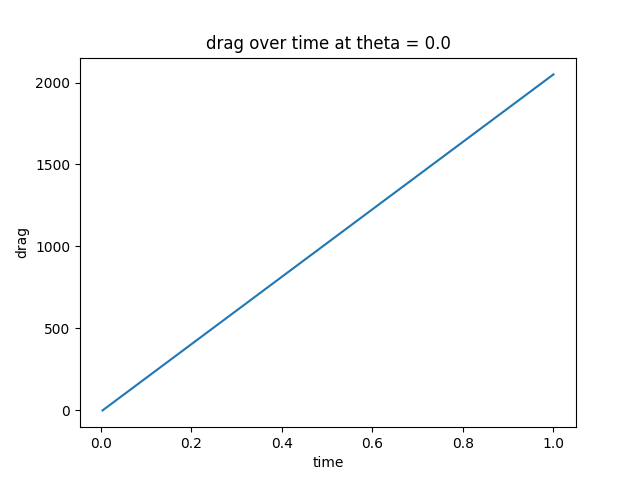
\includegraphics[scale=0.5]{../lift_and_drag/drag_0_0.png}
		\end{subfigure}%
		~ 
		\begin{subfigure}[t]{0.5\textwidth}
			\centering
			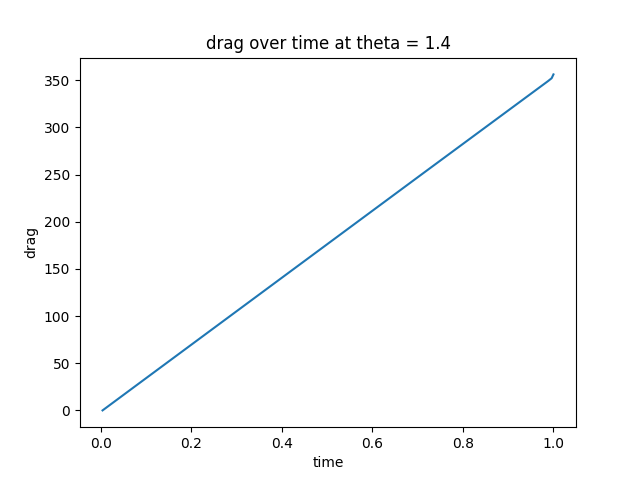
\includegraphics[scale=0.5]{../lift_and_drag/drag_1_4.png}
		\end{subfigure}
		\caption{Values for Drag vs. Time}
	\end{figure}

	They both display a linear relationship of drag over time. However, at $\theta = 1.4$, the maximum drag is significantly less than for $\theta = 0.0$.
	
	\begin{figure}[H]
		\centering
		\begin{subfigure}[t]{0.5\textwidth}
			\centering
			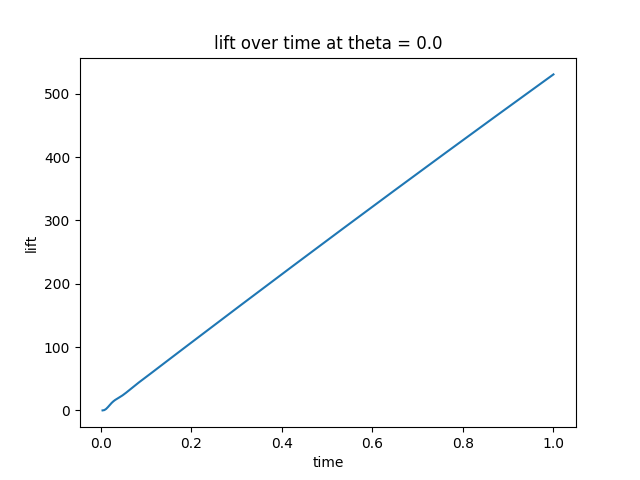
\includegraphics[scale=0.5]{../lift_and_drag/lift_0_0.png}
		\end{subfigure}%
		~ 
		\begin{subfigure}[t]{0.5\textwidth}
			\centering
			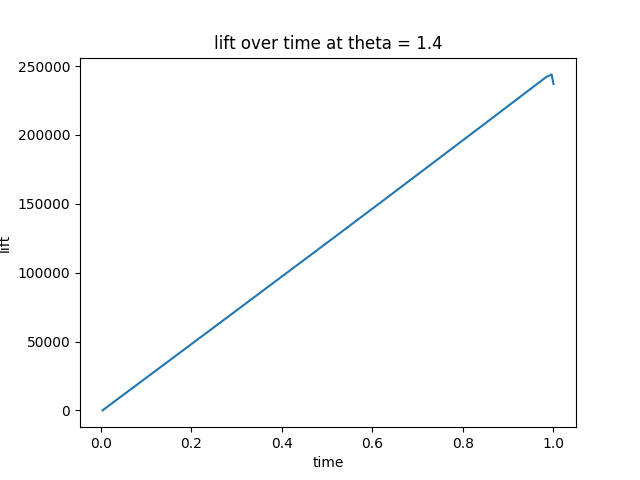
\includegraphics[scale=0.5]{../lift_and_drag/lift_1_4.png}
		\end{subfigure}
		\caption{Values for Lift vs. Time}
	\end{figure}

	Again, there is almost linear relationship between lift and time and there is an increase in maximum lift at higher values of $\theta$. It is interesting for $\theta = 1.4$, the lift drops off right around one second. 
	
	The next two plots show how the maximum lift and drag change with $\theta$.
	\begin{figure}[H]
		\centering
		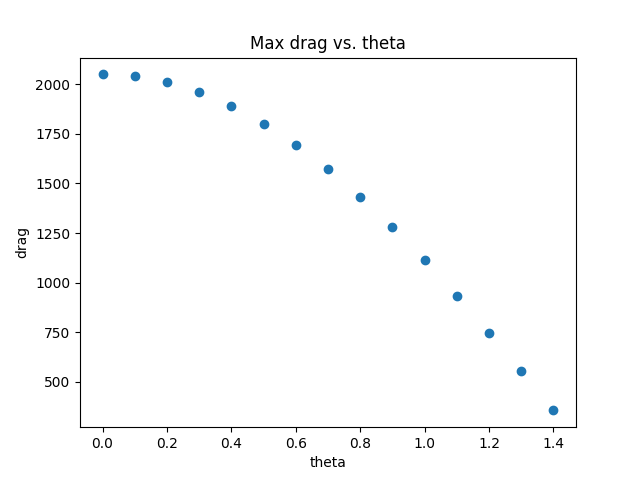
\includegraphics[scale=0.4]{../maxdrag.png}
		\caption{}
	\end{figure}
	\begin{figure}[H]
		\centering
		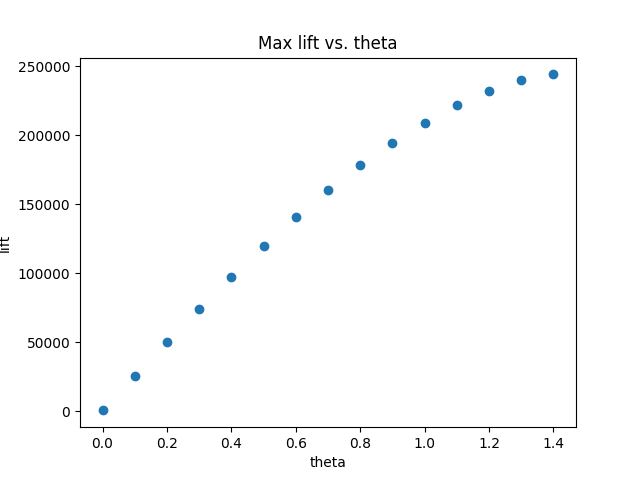
\includegraphics[scale=0.4]{../maxlift.png}
		\caption{}
	\end{figure}

	Here, we see that lift and drag have the opposite change as $\theta$ increases and in both cases, it makes sense. Note that $\theta = 0.0$ can be though of as being air flowing head on to the leading edge and $\theta = 1.4 \approx \pi/2$ as  air flowing from below. Then, it makes sense there would be more drag along against the leading edge if the air is coming head on at $\theta  = 0.0$ than when it is coming from below. Conversely, it makes sense that there is more lift if the air is coming from below at $\theta = 1.4$ then from head on.
	
	\begin{figure}[H]
		\centering
		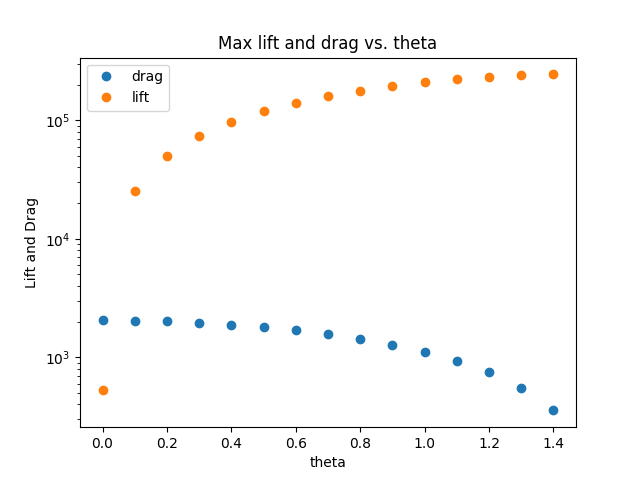
\includegraphics[scale=0.5]{../max_both.png}
		\caption{Lift vs. $\theta$ on a log-linear scale and drag vs. $\theta$ on a linear-linear scale}
		\label{fig:dragandlift}
	\end{figure}
	In \cref{fig:dragandlift} we see lift and drag vs. $\theta$ together. However, since lift is plotted on a log-linear scale, it is clear that the affects on lift are much greater as $\theta$ changes than for drag.
	
	There are a number of .xdmf files in the \textit{/navier\_stokes\_airfoil} folder that provide animations for the velocity and pressure over time for various $\theta$ values. However, I was unable to export them and embed them in this writeup due to issue with Paraview.
	
	\section*{Future Work}
	In the future, the first thing I would do is to develop a better understanding of the physics behind fluid dynamics. At the moment, I am not able to accurately verify that my results seems reasonable since I do not understand the underlying dynamics well enough. 
	
	Another avenue to explore is how changing the boundary condition on the right wall would affect the end result. I know that what type of condition imposed here can affect the solution upstream so it would be interesting to see what type of changes occur. 
	
	Another avenue of future work would be to compare different airfoils. Do they have different maximum lift and drags over different values of $\theta$? Would the equivalent of \cref{fig:dragandlift} look different for different airfoils?
	
	\bibliographystyle{unsrt}
	\bibliography{finproj}
	\section*{Appendix}
	\lstinputlisting[language=Python]{../generate_subdomains.py}
	\lstinputlisting[language=Python]{../flow_over_airfoil.py}
	
\end{document}